\documentclass{beamer}
\usepackage[latin1]{inputenc}

\usepackage[noend]{algpseudocode}
\usepackage[ruled]{algorithm}
\usepackage{url}
\usepackage{framed}
\usepackage{amsfonts,amsmath,amsthm}
\usepackage{graphicx}
\usepackage{url}
\usepackage{color}

\title{MCTS Based on Simple Regret}
\author{David Tolpin, Solomon Eyal Shimony}
\institute{Ben-Gurion University of the Negev\\Beer Sheva, Israel}
\date{February 22, 2012}

\AtBeginSection[]
{
  \begin{frame}<beamer>
    \frametitle{Outline}
    \tableofcontents[currentsection]
  \end{frame}
}


\begin{document}

\begin{frame}
\titlepage
\end{frame}

\begin{frame}{Hard to solve search problems}
Search problems are often hard too solve in practice when:
\begin{itemize}
\item search space is extremely large;
\item {\it and} good heuristics are unknown.
\end{itemize}
\textbf{Easier} to solve:
\begin{itemize}
\item Chess --- search space size is manageable ($10^{50}$).
\item Timetabling --- good heuristics.
\end{itemize}
\textbf{Hard} to solve:
\begin{itemize}
\item Compute Go ($10^{180}$), Poker ($10^{70}$).
\item Canadian Traveller Problem.
\end{itemize}
\end{frame}

\begin{frame}{MCTS}

{\bf M}onte {\bf C}arlo {\bf T}ree {\bf S}earch helps in large search spaces.
\begin{itemize}
\item Starts with the root only.
\item Repeats:
  \begin{enumerate}
    \item \textbf{Selection:} select a branch to explore.
    \item \textbf{Expansion:} adds children of the leaf to the stored
      tree.
    \item \textbf{Simulation:} continues search (using a simple
      strategy) until a goal state is reached.
    \item \textbf{Backpropagation:} values of each stored node 
      are updated.
  \end{enumerate}
\end{itemize}
\textbf{Adaptive} MCTS samples `good' moves more frequently,\\
but sometimes {\bf explores} new directions.
\end{frame}

\begin{frame}{Multi-armed Bandit Problem and UCB}
Multi-armed Bandit Problem:
\begin{itemize}
\item We are given a set of $K$ arms.
\item Each arm can be pulled multiple times.
\item The reward is drawn from an {\bf unknown} (but normally {\it
    stationary} and {\it bounded}) distribution.
\item The {\bf total reward} must be maximized.
\end{itemize}

{\bf UCB} is near-optimal for MAB --- solves
{\it exploration/exploitation} tradeoff.
\begin{itemize}
\item pulls an arm that maximizes {\bf U}pper {\bf C}onfidence {\bf
    B}ound: $b_i=\overline X_i+\sqrt {\frac {c \log (n)} {n_i}}$
\item the cumulative regret is $O(\log n)$.
\end{itemize}
\end{frame}

\begin{frame}{UCT}
UCT ({\bf U}pper {\bf C}onfidence Bounds applied to {\bf T}rees) is 
based on UCB.
\begin{itemize}
\item Adaptive MCTS.
\item Applies the UCB selection scheme at each step of the rollout.
\item Demonstrated good performance in Computer Go (MoGo, CrazyStone, Fuego,
  Pachi, ...) as well as in other domains.
\end{itemize}
However, the first step of a rollout is different:
\begin{itemize}
\item The purpose of MCTS is to choose an action with the greatest utility.
\item Therefore, the {\bf simple regret} must be minimized.
\end{itemize}
\end{frame}

\begin{frame}{SRCR}

{\bf S}imple {\bf R}egret followed by {\bf C}umulative {\bf R}egret.
\begin{itemize}
\item Maximizes {\bf simple regret} at the {\bf first step}.
\item Continues with UCT from the {\bf second step on}.
\end{itemize}
\vspace{1em}
\begin{algorithmic}[1]
\Procedure{Rollout}{node, depth=1}
  \If {\Call{IsLeaf}{node, depth}}
    \State \textbf{return} 0
  \Else
    \State \textbf{if} depth=1 \textbf{then} action $\gets$ \Call{FirstAction}{node} \label{alg:srcr-first-action}   
    \State \textbf{else} action $\gets$ \Call{NextAction}{node} \label{alg:srcr-next-action}
    \State next-node $\gets$ \Call{NextState}{node, action}
    \State reward $\gets$ \Call{Reward}{node, action, next-node}
     \State \hspace{4em} + \Call{Rollout}{next-node, depth+1}
    \State \Call{UpdateStats}{node, action, reward}
  \EndIf
\EndProcedure
\end{algorithmic}
\end{frame}

\begin{frame}{Sampling for Simple Regret}
Sampling schemes for miniminizing the simple regret:
\begin{enumerate}
\item $\varepsilon$-greedy sampling.
\item a modified version of UCB (worse for cumulative, better for
  simple regret).
\item<+-> VOI-based sampling.
\end{enumerate}

\begin{itemize}
\item<+-> 1, 2 --- heuristic selection criterion, theoretical upper bounds
  can be obtained.
\item<+-> 3 --- based on principles of {\it Rational Metareasoning},
  but harder to analyze.
\end{itemize}

\end{frame}


\begin{frame}{Doing better than UCT on sets}
\begin{figure}[h]
\centering
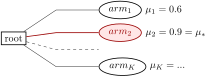
\includegraphics[scale=0.8]{onelevel-tree.pdf}
\end{figure}
When an arm is selected based on the {\bf sample mean}:
\begin{itemize}
\item Regret of UCB decreases {\it polynomially} with $n$.
\item Regret of $\epsilon$-greedy decreases {\it exponentially} with
  $n$.
\item Regret of UVB: $\max V_i$, $V_{i_{best}}=\frac {1-1/k}
  {n_{i_{best}}},\quad V_{i_{other}}=\frac {1/k} {n_{i_{other}}}$
  decreases exponentially with $n$, faster than $\epsilon$-greedy.
\end{itemize}
\end{frame}

\begin{frame}{UCB vs. $\epsilon$-greedy vs UVB}
\begin{figure}[h]
\centering
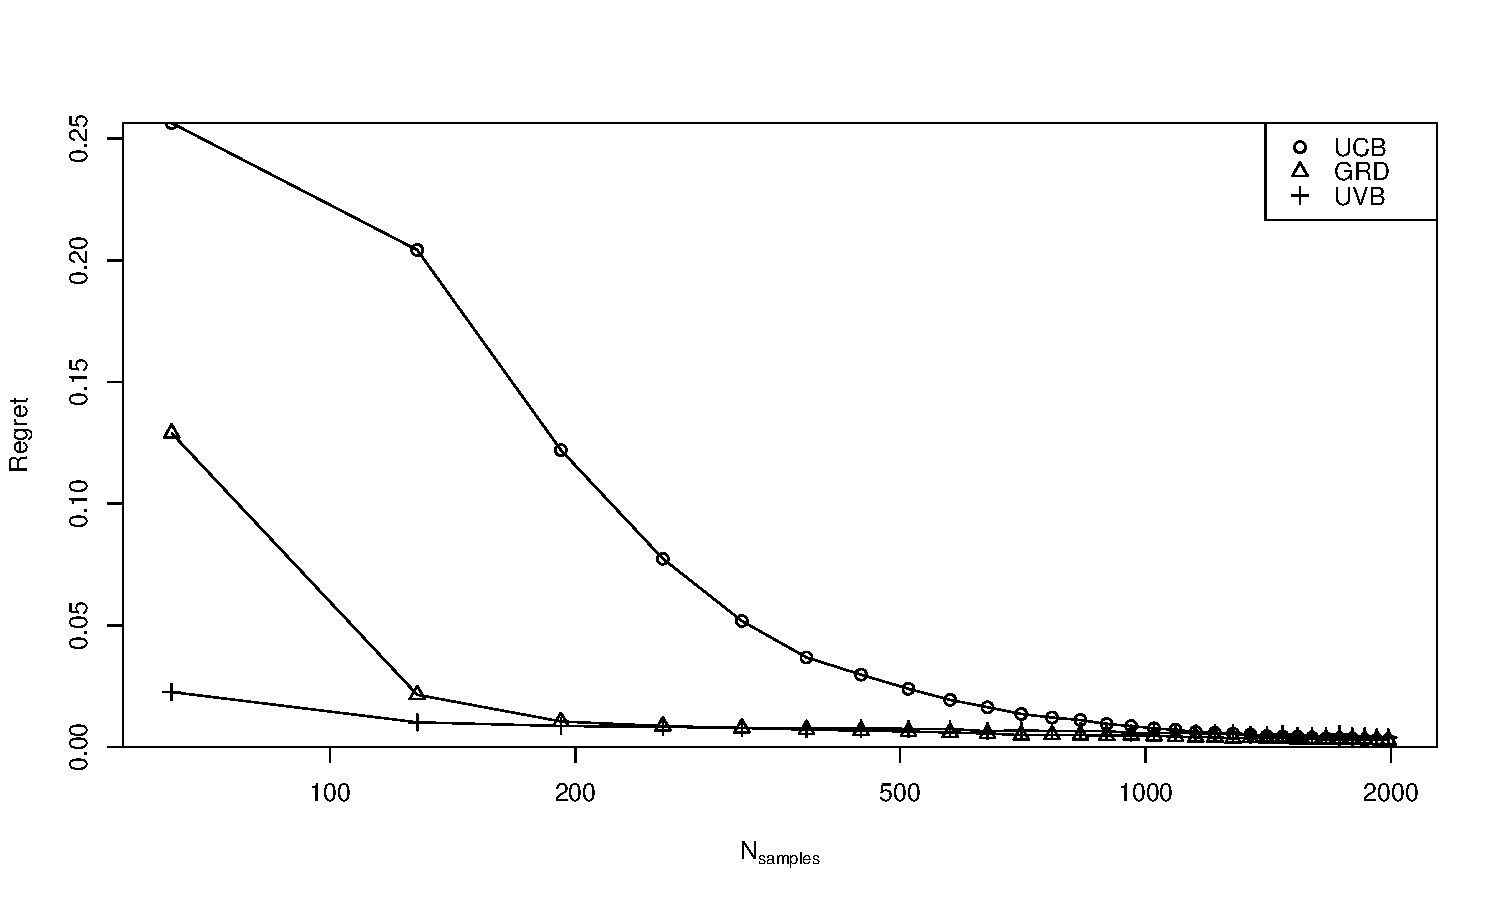
\includegraphics[scale=0.45]{onelevel-64.pdf}

64 Bernoulli arms, randomly generated
\end{figure}
\end{frame}

\begin{frame}{Doing Better Than UCT on Trees}
Uniform sampling is useless in this tree:
\begin{figure}[h]
\centering
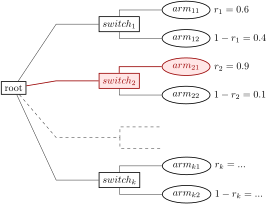
\includegraphics[scale=0.8]{twolevel-tree.pdf}
\end{figure}
Rational sampling:
\begin{itemize}
\item first, choose an action that maximizes VOI (UVB);
\item then, choose actions that maximize average reward (UCB).
\end{itemize}
\end{frame}{}

\begin{frame}{UVT vs. VCT (UVB+UCT) vs. UCT}
\begin{figure}[h]
\centering
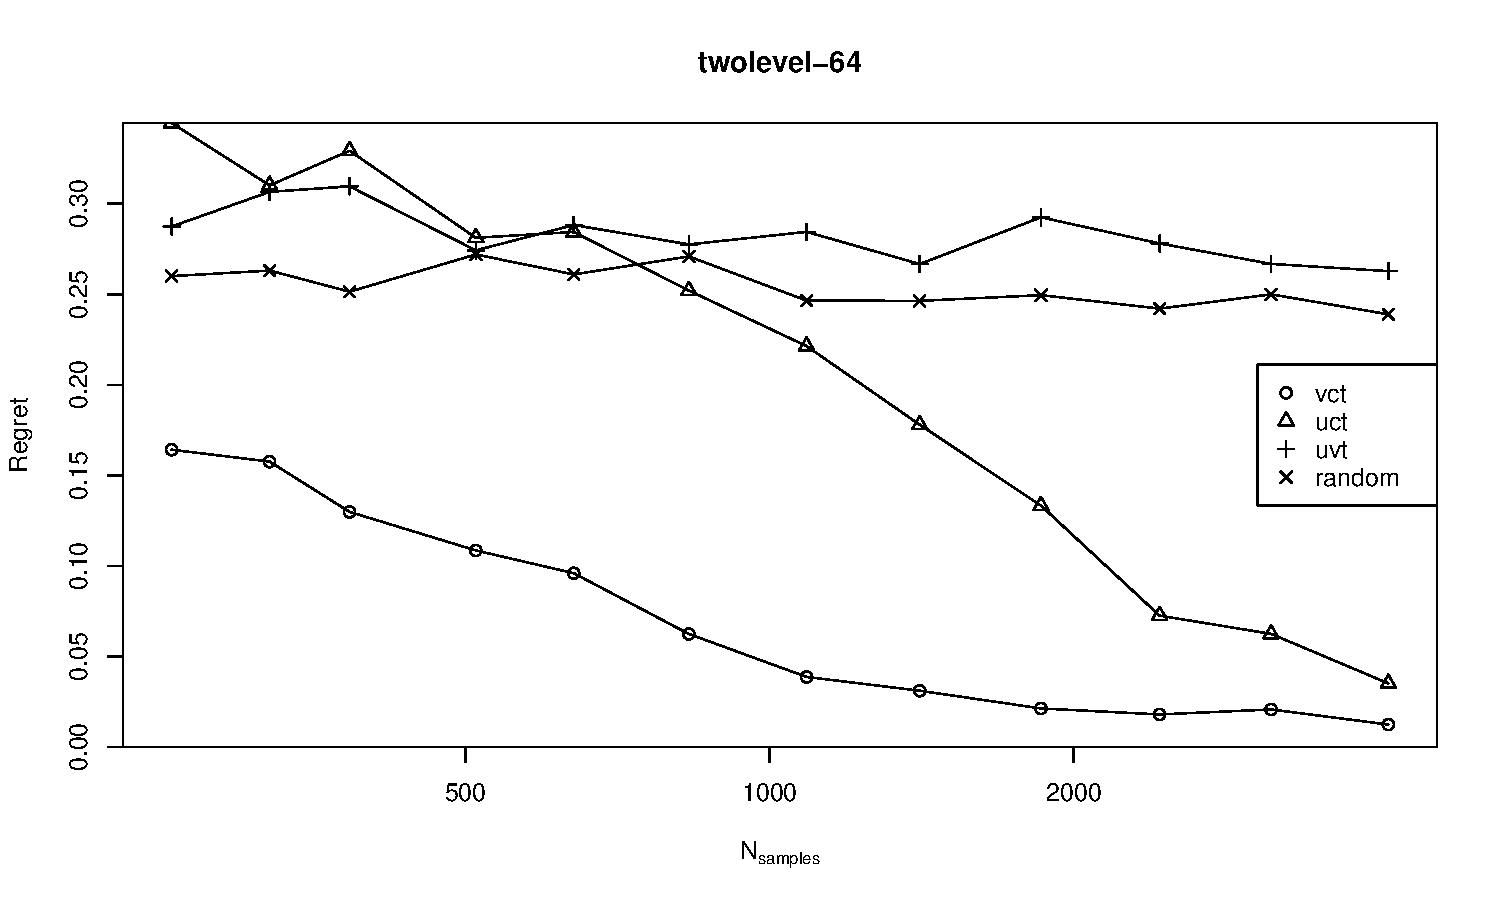
\includegraphics[scale=0.45]{twolevel-64.pdf}

64 Bernoulli arms, randomly generated
\end{figure}
\end{frame}

\end{document}
